
%(BEGIN_QUESTION)
% Copyright 2013, Tony R. Kuphaldt, released under the Creative Commons Attribution License (v 1.0)
% This means you may do almost anything with this work of mine, so long as you give me proper credit

This pictorial diagram shows the wiring connections for a simple pressure control loop, where a loop-powered 4-20 mA pressure transmitter sends a signal to a Honeywell controller, which in turn sends another 4-20 mA signal to a control valve:

$$\includegraphics[width=15.5cm]{i02697x01.eps}$$

If an operator informs you that the control valve refuses to open even in manual mode, what types and locations of electrical faults might you suspect?  Are there any non-electrical faults which might also cause this to happen?


\underbar{file i02697}
%(END_QUESTION)





%(BEGIN_ANSWER)

If the valve will not open, it means either a mechanical failure is preventing upward motion of the valve stem, or something is preventing air pressure from reaching the valve actuator.  Possible faults include either an open or a short in the cable between the I/P and the controller.  A dead controller (failed output, or failed AC power supply to the controller) could cause this as well.
 
\vskip 10pt

Possible non-electrical faults include failed air supply to the I/P, plugged air line between I/P and valve, and a shut block valve at the supply port of the I/P.

\vskip 10pt

No fault in the transmitter (input) circuit would have any effect on the controller's output in manual mode, since the valve control circuit is independent of the transmitter circuit.

%(END_ANSWER)





%(BEGIN_NOTES)


%INDEX% Pictorial circuit review (4-20 mA loop)
%INDEX% Troubleshooting review: electric circuits

%(END_NOTES)


